\documentclass[a4paper, notitlepage]{article}

\usepackage{hyperref}
\usepackage[T1]{fontenc}
\usepackage{lmodern}
\usepackage{listings}
\usepackage{capt-of}
\usepackage{graphicx}
\usepackage{deluxetable}





\newcommand{\flame}{\texttt{flame}}
\newcommand{\fuel}{\texttt{fuel}}
\newcommand{\inp}{\texttt{input}}

\begin{document}

\lstset{language=IDL}

\title{\flame\ user manual}
\author{Sirio Belli}
\maketitle



% ***********************************************************************************************
% ***********************************************************************************************
%									1. INTRODUCTION
% ***********************************************************************************************
% ***********************************************************************************************


\section{Introduction}
\label{sec:introudction}

\flame\ is a pipeline for reducing near-infrared multi-object spectroscopic data, written in IDL. Although created specifically for the LUCI instrument at LBT, it has been designed in a modular way and can be easily adapted to work with the data produced by different instruments. The present document describes in detail the reduction of LUCI data. Section \ref{sec:other_instruments} summarizes the different settings needed for the reduction of data taken with different instruments.





% ***********************************************************************************************
% ***********************************************************************************************
%									2. INSTALLATION
% ***********************************************************************************************
% ***********************************************************************************************



\section{Installation}
\label{sec:installation}


\subsection{Requirements}

The following three external IDL libraries must be installed before running \flame.
\begin{enumerate}
\item NASA's \href{http://idlastro.gsfc.nasa.gov/}{IDL Astronomy User's Library};
\item David Fanning's \href{http://www.idlcoyote.com/code_tips/installcoyote.php}{Coyote Library};
\item Craig Markwardt's \href{https://www.physics.wisc.edu/~craigm/idl/fitting.html}{mpfit} (only the mpfit.pro and mpfit2dfun.pro files are needed).
\end{enumerate}
Make sure to have the most recent versions of these libraries (at least more recent than the January 2016 release).

Other third-party routines used by \flame\ are included in the distribution, in the flame/lib/ directory. These are the B-spline routines from the \texttt{idlutils} library, the L.A.Cosmic routine written by Joshua Bloom and Pieter van Dokkum, and the readmhdufits routine written by Marc Kassis.


\subsection{Download}

Download the \flame\ IDL code from \url{http://siriobelli.github.io/flame/}. Either save it in the directory where you keep your IDL code, or add the flame/ directory to the IDL path. No other step is necessary.





% ***********************************************************************************************
% ***********************************************************************************************
%									3. SETUP
% ***********************************************************************************************
% ***********************************************************************************************


\newpage

\section{Setting up the Data Reduction}
\label{sec:setup}


\subsection{Basic input}

Go to the directory that you want to use for the reduction of a data set (it is recommended to create a new directory for this purpose). Then:
\begin{itemize}
\item Copy the file \texttt{flame\_driver\_luci.pro} from the flame/pro/ directory to the current directory.
\item Create an ASCII file (e.g., science.txt) with, in each line, the full name (including absolute path) of a raw science file.
\item \emph{(optional)} Create additional ASCII files with the names of the calibration frames (e.g., darks.txt, flats.txt, etc.)
\end{itemize}

The data reduction is entirely controlled via the driver file. Open the local copy with a text editor and have a look at the code. The driver file is divided into three parts. The first part is where the input parameters are set; the second part is the initialization, and the third part is the data reduction. In this section we discuss the first part.

The first step in the driver file creates the \inp\ structure:
\begin{lstlisting}
 input = flame_create_input()
\end{lstlisting}
We now need to populate the fields in the \inp\ structure with values that are appropriate for the data set that we are reducing.
We start by specifying the name of the file containing the science frames; for example like this:
\begin{lstlisting}
input.science_filelist = 'science.txt'
\end{lstlisting}

In the near-infrared the observations are usually spatially dithered for an effective sky subtraction. \flame\ supports a two-point dithering, also called AB dithering, which is activated via the flag:
\begin{lstlisting}
input.AB_subtraction = 1
\end{lstlisting}

When observing faint targets, it is recommended to place a slit on a relatively bright star (hereafter called the reference star) from which the conditions and the spatial dithering can be accurately measured. In the AB dithering scheme, the star trace will appear on two different positions, which may be in the same slit or in two different slits. The y pixel position of the reference star in both the A and the B position must be provided:
\begin{lstlisting}
input.star_y_A = 547
input.star_y_B = 560
\end{lstlisting}
These coordinates do not need to be exact. If the trace is very faint in a single frame, a simple A-B subtraction is generally sufficient for a visual detection. When no reference star is available, the dithering pattern must be specified manually (see Section \ref{sec:troubleshooting}). If no AB dithering is performed, the B star position should be set to zero.

While the default behavior is to reduce all the slits in the mask, it is sometimes preferable to reduce only one slit, for example to obtain a quick reduction of a representative object while observing. This can be achieved by specifying:
\begin{lstlisting}
input.reduce_only_oneslit = 2
\end{lstlisting}
where in this case we would get the reduction of only the second slit. The default value is zero which means that all the slits will be reduced.

Finally, to reduce longslit observations, it is sufficient to set the longslit flag:
\begin{lstlisting}
input.longslit = 1
\end{lstlisting}
Because the longslit spans the whole detector in the vertical range, the edges of the longslit are not well defined. This means that the slit curvature cannot be traced, and the spatial distortion cannot be rectified. The region of interest must be specified by providing the y pixel coordinates of the top and bottom limits:
\begin{lstlisting}
input.longslit_edge = [1050, 1350]
\end{lstlisting}
If longslit\_edge is set to [0,0], the default is to reduce the full frame excluding 10\% of pixels at the bottom and 10\% at the top. For example, for a frame that is 2048 pixels tall, this would correspond to the [205, 1843] range.


\subsection{Advanced options}

The \inp\ structure contains additional fields that can be used to specify advanced options. The full list is reported in Table \ref{tab:input}. The expanded driver file \texttt{flame\_driver\_complete.pro} includes all the options: the relevant lines can be copied and then pasted in the local copy of the driver.

The calibration data are supplied to the pipeline via ASCII files containing a list of FITS files, similarly to what done for the science data:
\begin{lstlisting}
input.dark_filelist = 'dark.txt'
input.pixelflat_filelist = 'pixelflat.txt'
input.illumflat_filelist = 'none'
input.arc_filelist = 'none'
input.slitflat_filelist = 'none'
\end{lstlisting}
Each of these fields can be set to \textquoteleft none\textquoteright\ (no calibration applied), or to a text file containing the user-supplied calibration frames (such as \textquoteleft dark.txt\textquoteright).


\begin{deluxetable}{lll}
\tabletypesize{\footnotesize}
\tablewidth{0pc}
\tablecaption{Content of the \inp\ structure \label{tab:input}}
\tablehead{
\colhead{Field} & \colhead{Default Value} & \colhead{Description} }
\startdata
science\_filelist   	     & science.txt 		& name of ASCII file containing the list of science frames \\
AB\_subtraction      & 1      & flag to enable AB subtraction \\
input.star\_y\_A 		 & 0			& pixel y-coordinate of the A position of the star trace \\
input.star\_y\_B 		 & 0			& pixel y-coordinate of the B position of the star trace \\
reduce\_only\_oneslit 	& 0 				& if non-zero, reduce only that one slit \\
longslit 				& 0 				& set to one to reduce long-slit data \\
longslit\_edge			& [0, 0] 			& when reducing long-slit data, only consider this range of pixel y-coordinate \\
dark\_filelist   		       & none 				& name of ASCII file containing the list of dark frames\\
pixelflat\_filelist        & none 				& name of ASCII file containing the list of frames for pixel flat field	\\
illumflat\_filelist   		 & none 				& name of ASCII file containing the list of frames for illumination flat field	\\
arc\_filelist   		  & none 				& name of ASCII file containing the list of lamp arc frames	\\
dither\_filelist   		& none 				& name of ASCII file containing the list of dither positions \\
slitflat\_filelist    & none        & name of ASCII file containing the list of slit flats \\
slitflat\_offset      & 0           & vertical offset in pixels between the slit flat and the science frames \\
slit\_position\_file  & none        & name of ASCII file containing the approximate y-coordinates of the slit edges \\
max\_slitwidth\_arcsec & 0          & threshold value of the slit width to identify the alignment boxes \\
intermediate\_dir		 & intermediate/		& directory that will contain the intermediate products \\
output\_dir				   & output/			& directory that will contain the final output
\enddata
%\tablecomments{Some comment here.}
\end{deluxetable}


It is advisable to always have a reference star on the multi-slit mask. When this is not possible, \flame\ cannot measure the dithering offset for each frame, and the dithering pattern needs to be saved in an ASCII file. The file must contain a number of lines equal to the number of science frames. Each line will have the value of the vertical offset, in arcseconds, corresponding to that frame (for example 5, -5, 5, -5, etc). Then the file name needs to be input in the \inp\ structure:
\begin{lstlisting}
input.startrace_y_pos = [0, 0]
input.dither_filelist = 'dither.txt'
\end{lstlisting}


% Next, we need to define the directories for intermediate and final outputs:
% \begin{lstlisting}
% input.intermediate_dir = 'intermediate/'
% input.output_dir = 'output/'
% \end{lstlisting}
% If these directories do not exist, they will be created by \flame. Note that these definitions use relative paths, but it is safer to always use absolute paths (e.g., /scr/observing/run\_1/mask\_1/output/).




\subsection{Initialization}

The data reduction in \flame\ consists of a series of steps, which are represented by individual routines. The information is carried from one routine to the next via the use of only one structure, named \fuel, which contains all the input parameters set by the user, together with all the internal variables.

Once the \inp\ fields have been specified, the \fuel\ structure must be created:
\begin{lstlisting}
fuel = flame_initialize_luci(input)
\end{lstlisting}
This will also check for potential errors in the inputs, and create the necessary directories.

The \fuel\ structure consists of five substructures:
\begin{itemize}
	\item fuel.input: a copy of the \inp\ structure created in the previous step;
	\item fuel.util: utility variables needed by \flame;
	\item fuel.instrument: instrument-specific information;
	\item fuel.diagnostics: diagnostics such as seeing and transparency for each of the science frames;
	\item fuel.slits: information relative to each slit, such as position on the detector and expected wavelength range.
\end{itemize}

Some of the fields in the \fuel\ structure are initially set to null pointers and will be created by successive steps.

During the initialization, relevant fields from the FITS header of the science files, such as band, central wavelength, and slit positions are read and saved. This is the only step during the data reduction where instrument-specific operations are performed. Since the remaining steps are common to all near-infrared MOS data, it is in principle easy to adapt \flame\ to a different instrument by simply writing the appropriate initialization module.





% ***********************************************************************************************
% ***********************************************************************************************
%									4. DATA REDUCTION
% ***********************************************************************************************
% ***********************************************************************************************



\section{Running the Data Reduction}
\label{sec:data_reduction}

Once the first part of the driver file has been edited, the data reduction is fully automatic. One way to run \flame\ at this point would be to execute the driver directly from the command line:
\begin{lstlisting}
idl flame_driver.pro
\end{lstlisting}
Another possibility, which allows some interaction and testing, is to copy line-by-line the content of the driver file onto an interactive IDL session. In this way one can explore the output files and the fuel structure after every step.

The second part of the driver file contains eleven steps or modules, which we are going to examine in detail in this section. Every module is an IDL routine whose name starts with \texttt{flame\_} and which is saved in a .pro file with the same name in the directory flame/pro/. All modules accept (and require) only one argument, which is the \fuel\ structure, so that the IDL code for each module looks the same:
\begin{lstlisting}
flame_modulename, fuel
\end{lstlisting}

Every module edits the fuel structure and/or outputs files in the intermediate directory. Only the last module, which creates the final results, saves the output files in the output directory.



% ---------------------------------------------------
\subsection{\texttt{flame\_diagnostics}}
\label{sec:diagnostics}

The first step produces important diagnostics which will be used by the other modules. These diagnostics can also be helpful to the user to assess the quality of the observations, and can be run in real time while observing, ideally after every new frame or frame pair has been taken.

\begin{figure}[htbp]
\centering
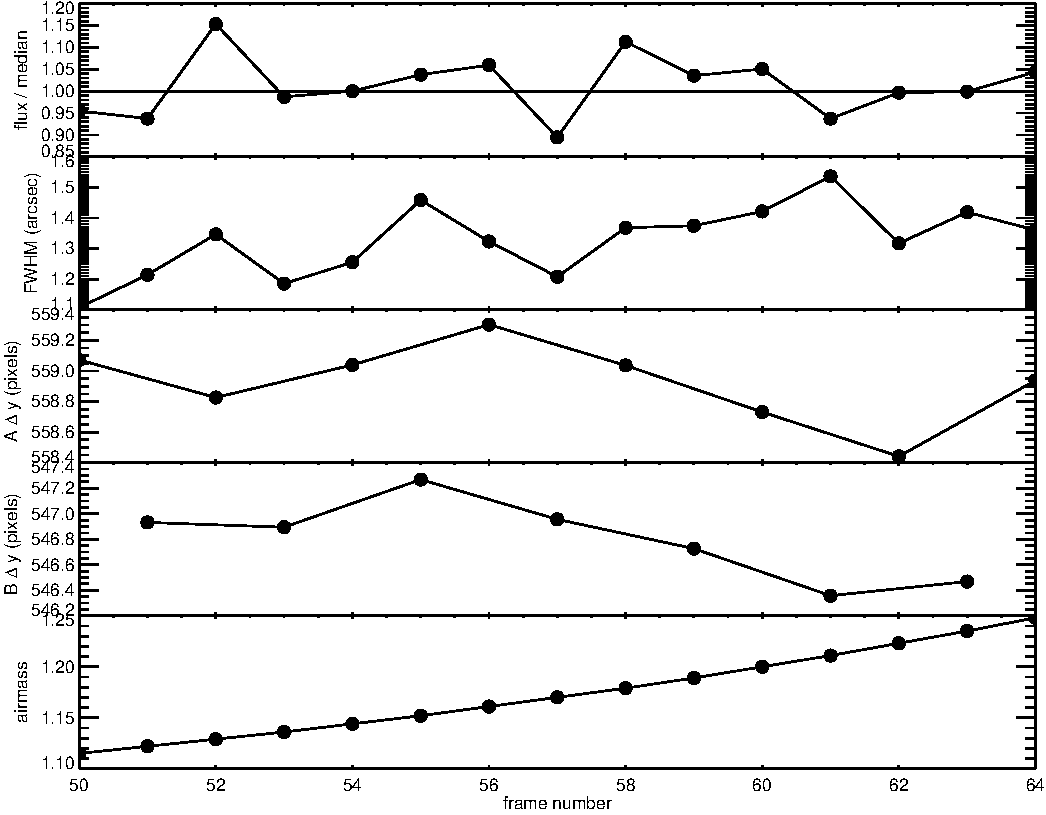
\includegraphics[width=0.9\textwidth]{diagnostics}
\caption{Example of diagnostic plots. From the top: Flux of the star trace, normalized by the median value; FWHM in arcsec; vertical position of the trace in A frames; vertical position of the trace in the B frames; airmass value read from the FITS header.}
\label{fig:diagnostics}
\end{figure}

Starting with the y coordinates specified by the user in fuel.startrace\_y\_pos, this module detects the reference star position on each frame, and identifies which frames belong to the $A$ and which to the $B$ position (and assign an $X$ position when no star trace is found). Then, for each frame a Gaussian profile is fit to the star trace, from which the flux, vertical position and FWHM are measured. In addition, the airmass value is read from the FITS header of each frame.

All these quantities are saved in the substructure fuel.diagnostics. They are also output in the ASCII file diagnostics.txt, and plotted as a function of the frame number in the file diagnostics.ps. One example of such file is shown in Figure \ref{fig:diagnostics}. Because of the dithering, the vertical position is shown in different panels for the $A$ and the $B$ frames. If there are multiple frames with same frame number, which can happen when combining data from different nights, then the x axis of the plot will show a sequential number (but the original frame numbers are used in the ASCII file).

The diagnostic plots can be used to judge the trend of transmission (including the effect of cloud cover), seeing, and drift. In addition to help the user make informed decisions while observing, these measurements are also useful to identify the bad frames that should be excluded from the final data reduction.



% ---------------------------------------------------
\subsection{\texttt{flame\_quickstack}}

The second step produces a FITS file which is the difference of a stack of the $A$ frames and a stack of the $B$ frames (as defined in the previous module). This step is also useful while observing, since the simple $A-B$ subtraction often yields a decent sky removal which allows the detection of faint continuum traces or emission lines.

The sole goal of this module is to allow a quick look at the data. This step can be skipped with no consequences for the remaining parts of the data reduction.



% ---------------------------------------------------
\subsection{\texttt{flame\_correct}}

This module applies a number of corrections to the raw science frames. First, the bad pixel mask is generated from the input dark and/or flat frames. If neither dark nor flat field frames were supplied, then the default bad pixel mask, stored in flame/data/, is used.

The following corrections are applied:
\begin{itemize}
\item Cosmic rays removal: this step is not recommended for near-infrared data, but can be necessary for observations in the optical.
\item Linearity correction: the value of each pixel is corrected to take into account the non-linear response of the detector. The correction is a polynomial function with instrument-specific coefficients, which are determined during the initialization.
\item Pixel flat field correction, if required.
\item Bad pixels are set to NaN.
\item The flux of each pixel is multiplied by the gain and divided by the exposure time. This converts the flux units from ADUs to electrons/second.
\end{itemize}

The corrected science frames are then saved in the intermediate/frames/ directory. Each FITS file contains a second extension with the error spectrum, which is calculated as the combination of read-out noise and Poisson noise.


% ---------------------------------------------------
\subsection{\texttt{flame\_getslits}}
\label{sec:getslits}

The module \texttt{flame\_getslits} is responsible for detecting the slits from the multi-object slitmask. The vertical coordinates of the slit edges calculated during the initialization are used. However, the physical position of the mask with respect to the detector is typically difficult to predict and varies slightly from one night to the other. To account for this, a vertical shift is calculated by identifying the slit edges.

Once the approximate pixel position of each slit has been calculated, a second, more refined slit edge detection is run. This is based on the identification of individual OH emission lines, which are typically very bright and can be reliably used to trace the edge of a slit. For each slit, a low-order polynomial is fit to the $y$ coordinate of the edge as a function of $x$ position, and the results are saved to the fuel structure. Note that this procedure is more likely to fail when the slits are short or when there is not much space between one slit and the next one. When observing in the $K$, the low number of OH lines and the strong continuum sky emission makes it convenient to use the sky background instead (see Section \ref{sec:use_sky_edge})

The output file slitim.fits is a mask image where the value of each pixel is an integer indicating the slit number to which that pixel belongs to, with zero indicating pixels that do not belong to any slit. Also, the file slits.reg is saved, which is a ds9 region file that can be loaded on top of any science frame and will show the slit edges (see Figure \ref{fig:slits}). This can be used to check the slit detection and also to identify which slit on the science frame corresponds to which target.

\textbf{Explain the option of manually specifying the slit edges for difficult cases.}

\begin{figure}[htbp]
\centering
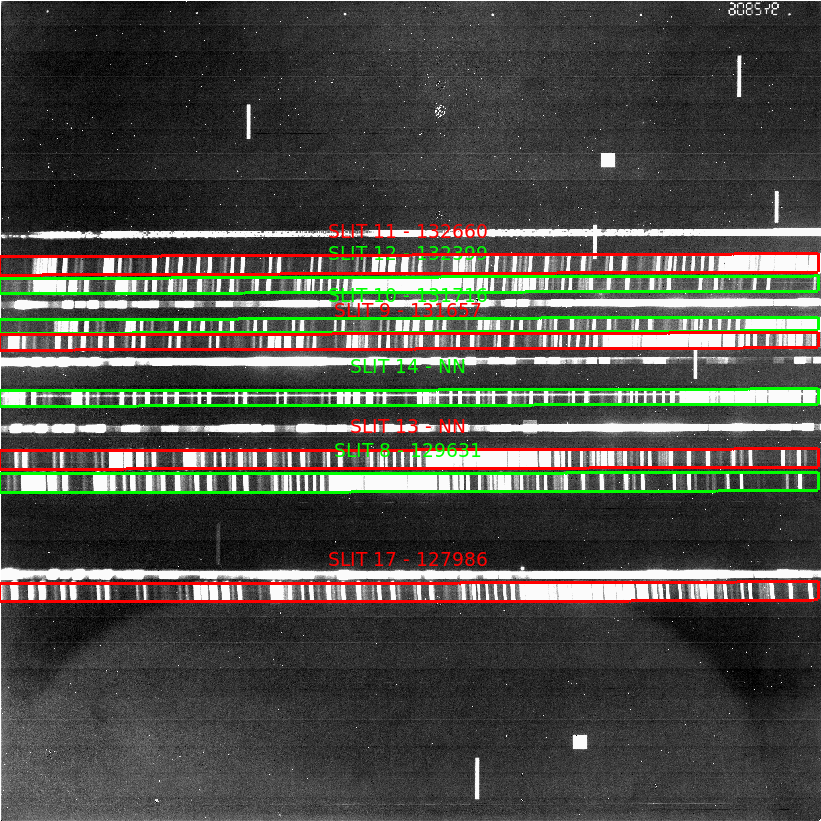
\includegraphics[width=0.7\textwidth]{slits}
\caption{An example of LUCI raw frame, with the regions marking the slits identified by \flame\ shown in green. The slits that are not marked are the boxes for the alignment stars, which are ignored by the pipeline.}
\label{fig:slits}
\end{figure}


% ---------------------------------------------------
\subsection{\texttt{flame\_cutout\_slits}}

Using the slit definition from the previous step, the slits are extracted from each corrected frame and saved as FITS files. All the cutouts corresponding to the same slit are saved in the directory slitxx, where xx is the slit number.


% ---------------------------------------------------
\subsection{\texttt{flame\_wavecal\_rough}}

The wavelength calibration is arguably the most important and difficult step in the data reduction. An accurate calibration is not only useful for the scientific interpretation of the data, but is also necessary for a correct sky subtraction.

In \flame, the wavelength calibration is split into three steps. The first step finds an approximate wavelength calibration for the central part of the slit, using only the first science frame. The sky spectrum is extracted from the central five pixels of the slit, and is compared to a model spectrum. The comparison consists of two successive steps:
\begin{enumerate}
\item Both the observed and the model sky spectra are smoothed to an intermediate spectral resolution ($R=500$, but this value is stored in the input structure and can be changed by the user), and a series of values for the pixel scale (in micron per pixel) are tested. At each loop, cross-correlation is used to find the initial wavelength, and the pixel scale that gives the largest value of the cross-correlation is selected.
\item Once the pixel scale and the initial wavelength are roughly known, a finer comparison is performed. In this case the spectra are not heavily smoothed, so that the narrow OH lines can be used for a very effective comparison. The relation between $x$ pixel coordinate and wavelength is typically not linear, and a second-order polynomial is used: $\lambda(x) = a_0 + a_1 x + a_2 x^2$. A fine grid of values for $a_1$ and $a_2$ is used, and at each loop cross-correlation is used to determine the best value for $a_0$.
\item Finally, another cross-correlation is performed at the native spectral resolution.
\end{enumerate}

For each slit, plots illustrating the successive comparisons of observed and model sky spectra are saved as ps files (wavelength\_solution\_estimate.ps). An example is shown in Figure \ref{fig:wavecal_approx}.

If the sky spectrum includes a strong contribution from continuum emission, as is often the case for the thermal emission in the K band, it may be necessary to fit and subtract a low-order polynomial to the observed spectrum before comparing it to the model. This can be done be setting \texttt{util.wavecal\_rough\_continuum\_degree} to a number different from zero, which will be taken as the degree of the polynomial representing the continuum (typically about five or less).


\begin{figure*}[tbp]
\begin{minipage}{\textwidth}
   \centering
 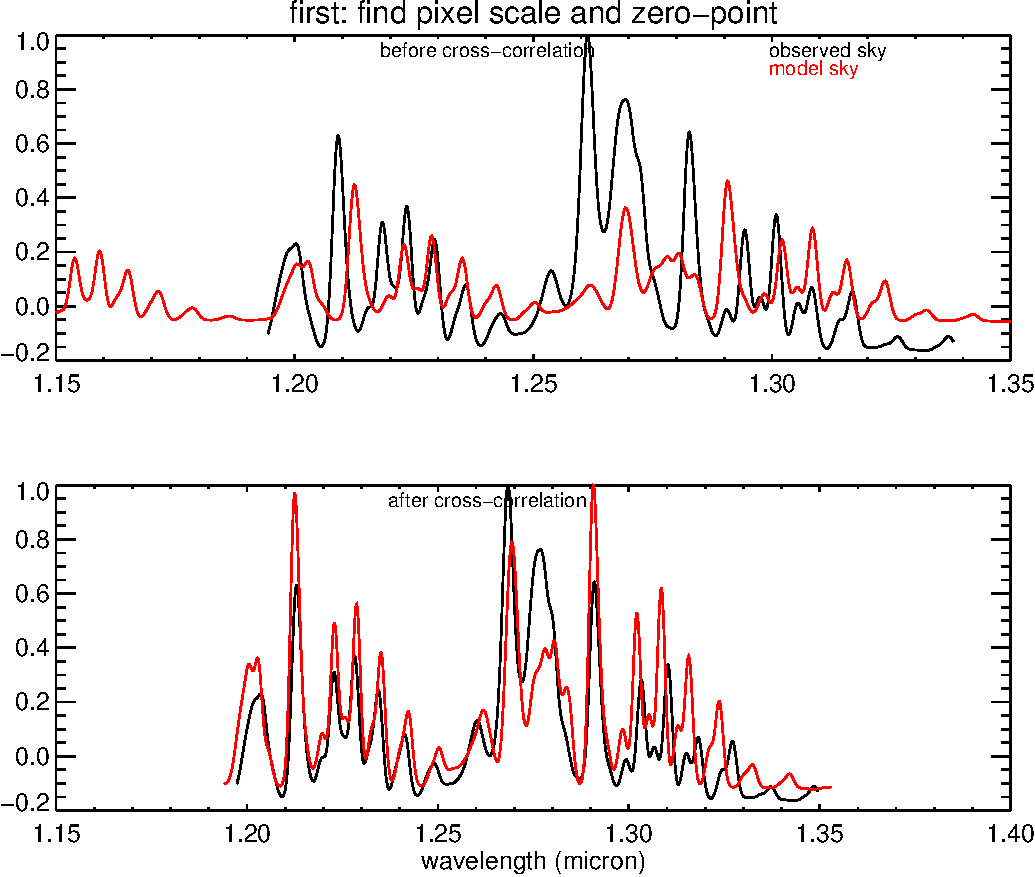
\includegraphics[width=0.31\textwidth]{wavecal1}
   \hspace*{0.01\textwidth}
 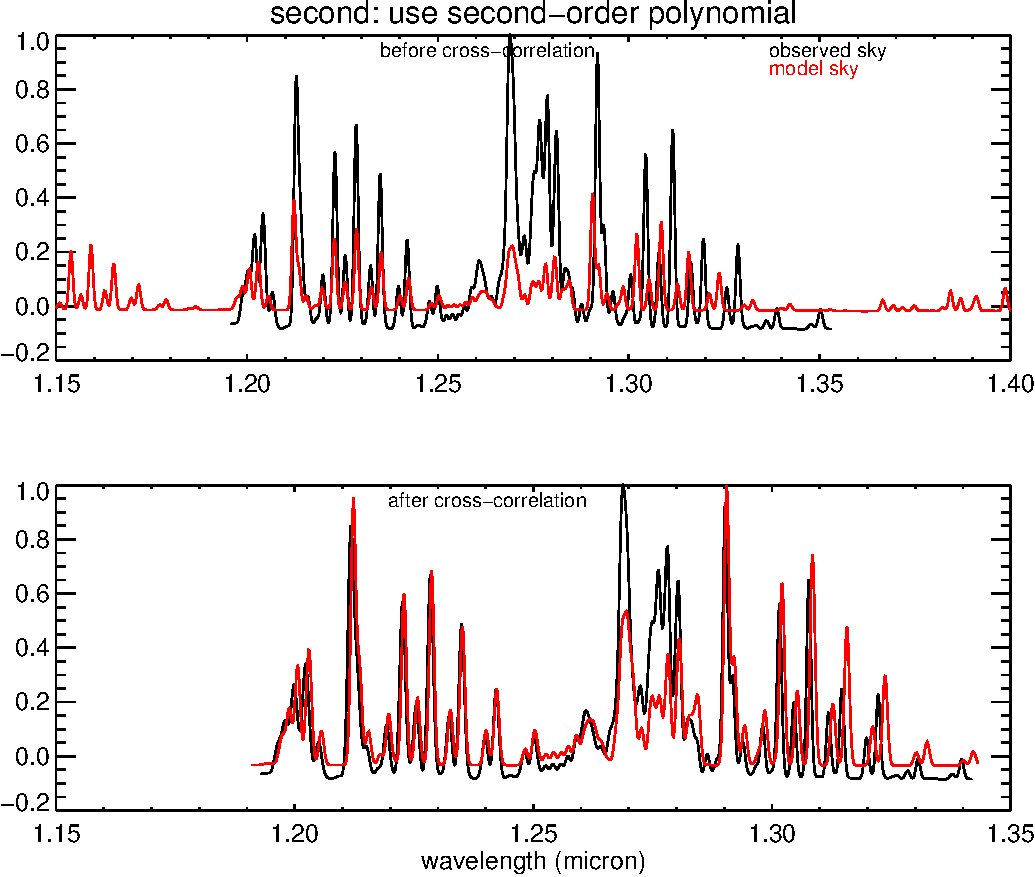
\includegraphics[width=0.31\textwidth]{wavecal2}
  \hspace*{0.01\textwidth}
 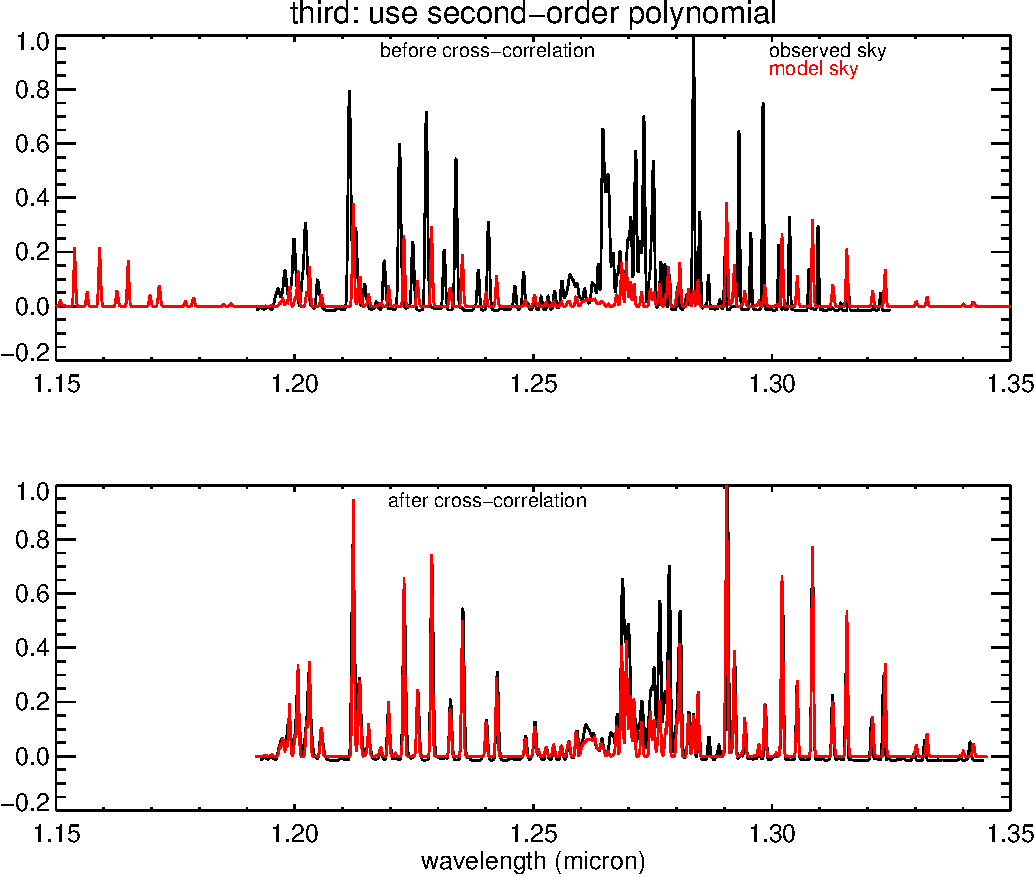
\includegraphics[width=0.31\textwidth]{wavecal3}
\end{minipage}
\caption{Approximate wavelength calibration. The sky spectrum (in black) is extracted from the central region of the slit, and is compared to a template spectrum (in red). The top panels show the initial guess, and the bottom panels show the results of the cross-correlation. The cross-correlation is repeated three times using successively higher spectral resolution.}
\label{fig:wavecal_approx}
\end{figure*}


% ---------------------------------------------------
\subsection{\texttt{flame\_identify\_lines}}


The previous procedure gives only a rough wavelength calibration that is valid for the pixel rows at the center of the slits. Since the wavelength solution typically varies with spatial coordinate within the slit (particularly for tilted slits), the calibration needs to be calculated for each individual pixel row, which is done in this step.

Initially, the spectrum of the central pixel row is extracted, and the individual OH emission lines are identified using the rough wavelength solution. A Gaussian fit is performed on each line, and the $x$ pixel coordinate corresponding to the center is stored. It is therefore necessary that the calibration found in the previous step is accurate to within the window used in the Gaussian fit, otherwise the identification of the OH lines will not be possible. The relation between the $x$ coordinate and the expected wavelength of each OH line is then fit with a low order polynomial (see example in Figure \ref{fig:speclines}). This procedure is then repeated for the next pixel row, using the wavelength solution from the previous pixel row as first guess. This is always a good assumption as long as the wavelength solution varies smoothly with position, without abrupt changes from one pixel position to the next.

After all the pixel rows have been processed, the final result is a number of $x,y$ coordinates of detected OH lines, and the corresponding theoretical wavelength. A ds9 region file (OHlines.reg) showing the detected location of the OH lines is produced.


\begin{figure}[tbp]
\centering
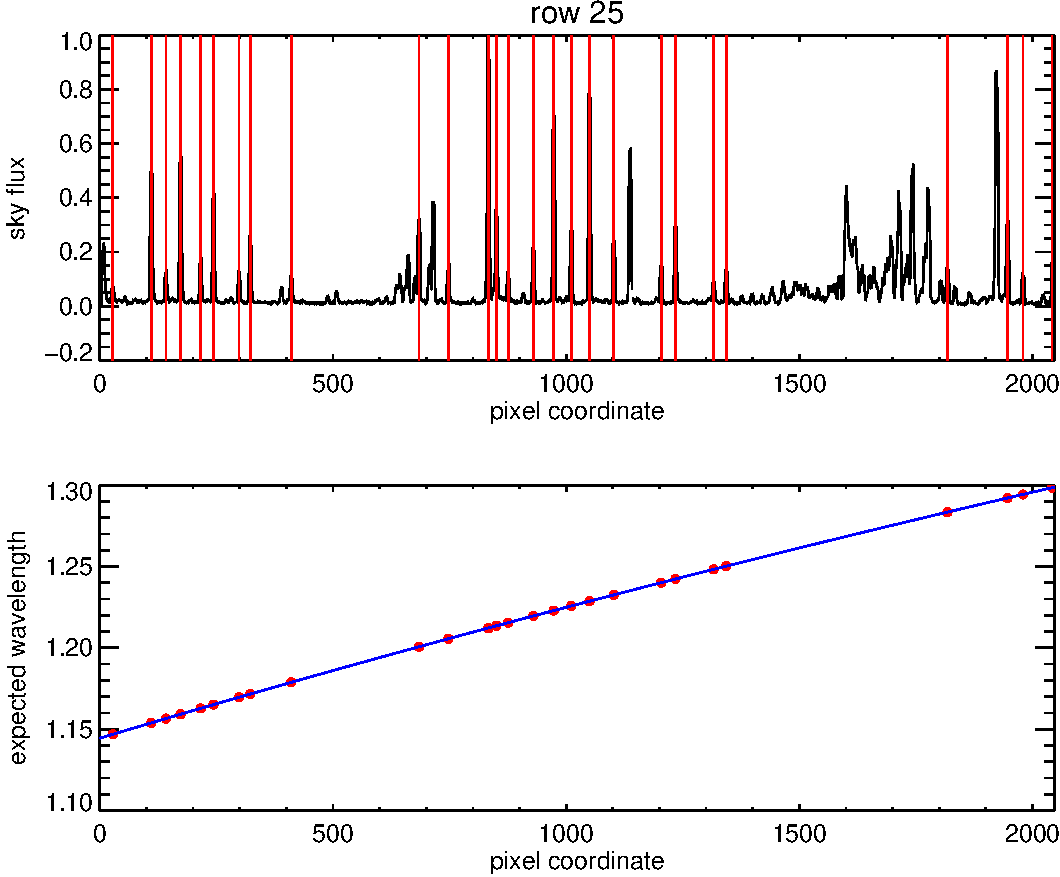
\includegraphics[width=0.7\textwidth]{wavecal_accurate}
\caption{Identification of sky lines. Top panel: The sky spectrum is extracted from a single pixel row, and using the approximate wavelength calibration the OH lines are identified and fit with a Gaussian profile. Bottom panel: the measured position of each OH line, together with their known wavelength, allow an accurate wavelength solution, shown in blue.}
\label{fig:speclines}
\end{figure}


% ---------------------------------------------------
\subsection{\texttt{flame\_wavecal\_accurate}}

For each sky line identification, we have a matching set of \emph{observed} pixel coordinates $(x,y)$ and \emph{rectified} coordinates $(\lambda,\gamma)$, where $\lambda$ is the theoretical wavelength of the OH line and $\gamma$ is simply the vertical distance (in pixels) from the bottom edge of the slit, calculated using the polynomial fits obtained by \texttt{flame\_getslits}. The wavelength solution and the


% ---------------------------------------------------
\subsection{\texttt{flame\_skysub}}

Because the OH emission lines vary on short timescales, the A-B subtraction typically leaves strong residuals. In order to improve the sky subtraction, \flame\ adopts the method of Kelson 2003. Briefly, the wavelength solution is used to map each pixel from the observed, distorted frame to the output, rectified frame. The distortion in the observed frame (which is produced by the optics and/or by the tilted slits) produces a very fine sampling of the sky lines in the rectified frame. Because of this sub-pixel sampling, it is possible to obtain an excellent B-spline fitting of the emission lines. \flame\ performs this operation on each frame for every slit, and saves a FITS file of the sky-subtracted data. A graphic window shows, during this step, the sky emission spectrum (collapsed onto one dimension) and the B-spline fit for every frame.


% ---------------------------------------------------
\subsection{\texttt{flame\_rectify}}

Using the 2D rectification coefficients calculated in \texttt{flame\_wavecal\_accurate}, this step performs both the wavelength calibration and the spatial rectification simultaneously, using only one interpolation. In practice, for each slit and each frame a polynomial warping is applied to the observed 2D spectrum, and a rectified FITS file is produced.


% ---------------------------------------------------
\subsection{\texttt{flame\_combine}}

The last step consists in the stacking (after sigma-clipping) of all the A and B frames. The individual A and B stacks, and the difference A-B, are output as FITS file for each slit. Non-skysubtracted versions of the stacks are also saved. Also, an ABcombined FITS file is produced by summing A-B to the shifted B-A images, so that one positive central trace, corresponding to the total observing time, can be extracted for the science analysis.

Sometimes the dithering is such that one object spends half of the time in one slit and half of the time in another slit. This is particularly useful when the slits need to be tilted in directions that are different from the dithering direction (as is the case when different objects in the mask require different position angles). If the dithering length, as calculated from the star traces, matches the distance between any two slits, then these are assumed to be matching slits and their A-B stacks are combined together. It is worth pointing out that this assumption breaks down if the star traces for the A and B positions actually belong to different stars.


% ***********************************************************************************************
% ***********************************************************************************************
%									5. TROUBLESHOOTING
% ***********************************************************************************************
% ***********************************************************************************************



\section{Troubleshooting}
\label{sec:troubleshooting}


\subsection{Bad fit to sky lines}

Sometime the sky lines are not bright or numerous enough for a reliable wavelength calibration. This can happen especially in the K band, where the OH lines are less numerous and the spectrum is typically dominated by thermal emission. Another situation where this issue can arise is when the OH lines are faint due to very short exposure times. In this cases it is always advisable to obtain arcs. There are however a few settings that can be optimized to obtain a satisfactory wavelength solution.

During the \texttt{flame\_identify\_lines} step, at each pixel row a polynomial is fit to the position of the sky lines (see Figure \ref{fig:speclines}). This part is critical and is often the first to fail in sub-optimal conditions. If the number of sky lines identified in one row is too low, the fit will not be considered valid. It is possible to change this threshold number by changing the variable \texttt{fuel.util.identify\_lines\_Nmin\_lines}. However, with a low number of lines it is also necessary to lwer the degree of the polynomial, to avoid over-fitting and obtaining meaningless wavelength solutions. This can be done by changing the variable \texttt{fuel.util.identify\_lines\_poly\_degree}.

Another possibility is to manually exclude those sky lines that are clearly problematic. This can be done easily by commenting out one or more entries in the line list, which is stored as a text file in the flame/data/ directory.


\subsection{Slit identification}

If the slit identification fails or is not accurate, one alternative is to use the longslit option to manually select the region within one slit to reduce. By default the longslit option assumes that the slit is spatially centered on the mask. If this assumption causes a wildly wrong initial guess for the wavelength range, it is possible to override this value by changing the \texttt{fuel.slits.range\_lambda0} variable, which is a 2-element array containing the minimum and maximum values to be considered for the wavelength of the first pixel.

Sometimes using a different science frame gives a better slit identification. The default frame used for the slit identification is the one in the middle; this file name is stored in \texttt{fuel.util.master\_getslit} and can be changed.


\subsubsection{Detection of slit edges with sky background}
\label{sec:use_sky_edge}

In some cases, particularly in the $K$ band, there are not enough bright OH lines for identifying the slit edges (see Section \ref{sec:getslits}). It is possible to use the continuum emission instead, by specifying
\begin{lstlisting}
input.trace_slit_with_skylines = 0
\end{lstlisting}


\subsubsection{Detection of slit edges with slit flat field}

If the slit edges are not well defined in the science frames, it is possible to use a flat field for the slit identification:
\begin{lstlisting}
input.trace_slit_with_skylines = 0
input.slitflat_filelist = 'slitflat.txt'
input.slitflat_offset = 4
\end{lstlisting}
where the file slitflat.txt contains a list of file names corresponding to the slit flat field data. These can be the same as the pixel and/or illumination flats.
It is often the case that the science frames present a vertical shift compared to the calibration frames because of flexure. In this case the shift needs to be measured manually and specified via the \texttt{slitflat\_offset} setting.


\subsection{Specify the x coordinates for the reference star}

When the reference star is present, its trace is extracted and used as a diagnostic tool (see Section \ref{sec:diagnostics}). Only the central part of the trace is used, in the interval [1000, 1200] in x-pixel coordinates. If the trace is too faint in this central region, it is possible to define a different range for the extraction:
\begin{lstlisting}
input.xrange_star = [100, 500]
\end{lstlisting}



\begin{deluxetable}{lll}
\tabletypesize{\footnotesize}
\tablewidth{0pc}
\tablecaption{Settings in the \texttt{fuel.util} structure \label{tab:util}}
\tablehead{
\colhead{Field} & \colhead{Default Value} & \colhead{Description} }
\startdata
star\_x\_range 			& [1000, 1200]		& range of star trace (in pixel x-coordinate) that will be extracted \\
rough\_wavecal\_R 	& 500				& target spectral resolution for the rough wavecal calibration \\
trace\_slit\_with\_skylines			& 1 				& if set, the slit detection is based on the sky emission lines instead of the continuum
\enddata
%\tablecomments{Some comment here.}
\end{deluxetable}



% ***********************************************************************************************
% ***********************************************************************************************
%									6. OTHER INSTRUMENTS
% ***********************************************************************************************
% ***********************************************************************************************

\section{Other instruments}
\label{sec:other_instruments}

\subsection{Keck LRIS}


% ***********************************************************************************************
% ***********************************************************************************************
%									CREDITS
% ***********************************************************************************************
% ***********************************************************************************************


\vspace{10mm}

\section*{Credits}

\flame\ was written by Sirio Belli with substantial help from Alessandra Contursi and Tom Fletcher for development and testing. Many features were inspired by code written by Eva Wuyts and Ric Davies for the LUCAS pipeline, and by Nick Konidaris' MOSFIRE DRP. Dave Thompson provided useful information particularly for the LUCI-specific parts.


\end{document}
